% Chapter 2

\chapter{Background} % Chapter title

\label{ch:background} % For referencing the chapter elsewhere, use \autoref{ch:background} 

%----------------------------------------------------------------------------------------

In this chapter, we are going to review about the history of the MLS, its definitions, usages, and one of its most famous models: the Bell-LaPadulla model.
MLS is a very famous solution for the old world security problems for multiple subjects accessing one shared system. 
Studying about it will open various paths to the information security solutions.
We can see how we can keep the system forcefully secured; 
how we can divide the system into different levels, each of which has corresponding policies, to archive the security requirements comprehensively.
\marginpar{In MLS systems, there are only \emph{subjects} and \emph{objects}, which have various \emph{properties} called \emph{clearance} and \emph{classification}} 
Moreover, MLS also defines objectively relations between multi-level users with the system's assets. 
Additionally, we also see how those advantages are designed in BLP model, as well as its ideas of an MLS system.

%----------------------------------------------------------------------------------------

\section{Multi-level Security}
\label{ch:background:mls}

Since the very early time of computer era, from 1960s, the need of communicating and sharing information among users in a same system was already tremendous.
Along with the raise of the number of services and connected devices, information security is becoming paramount in organizations, especially government's, intelligent agents, etc...
In the event such organizations' secret data is made public, it may lead to various level of damages.
In consideration of issues caused by the failure, \citeauthor{centos:2008} cited that:

\begin{quote}
Businesses may face legal or financial ramifications. At the very least, they will suffer a loss of customer trust. 
In most cases, however, they can recover from these financial and other losses with appropriate investment or compensation. 
The same cannot be said of the defense and related communities, which includes military services, intelligence organizations and some areas of police service.
These organizations cannot easily recover should sensitive information be leaked, and may not recover at all. 
\end{quote}

In every organizations, there's very likely a central system where everyone with different roles can login and access data flowing in it.
While some pieces of data are not so vital, they can be viewed or edited by anyone in the team, the others could be only essential to be available to a small group of particular people who are more influential, or in charge of making decisions.

According to \citeauthor{bancinco:2015} , under MLS, users and machine processes are called \emph{subjects}, and files, devices and other passive components of the system are called \emph{objects}.
So, MLS is a system design which allows multiple subjects (users) with difference clearance levels can access objects (data) flowing in the system while restricting their accesses corresponding to their clearance (or security level) \eg\ Unclassified, Confidential, Secret, Top Secret etc...
For example, in BLP model, in regard to reading permission, Secret subjects can only access to Secret or lower security level objects.

\begin{figure}[bth]                                                                                                                                                  
\myfloatalign
\includegraphics[width=1.0\linewidth]{gfx/chapter_2/security_level_read_example}
\caption[BLP: Security Levels read examples]{BLP: Security Levels read examples}\label{fig:security_level_read_example}
\end{figure}

Rather than that, a successful MLS system should allow various subjects to access and share objects, with acknowledge, to suitable others.
The objects' owners should not be in charge of making decision who they want to access to their assets individually, \citeauthor{prasun:1996} called this kind of control is \emph{discretionary access control}, because it is hard for the owner to manage when the number of his objects becomes huge or some of them are too old to remember, consequently causes data leaked or mis-used.
Hence, MLS design should \emph{force} subjects and all of their objects to follow an agreed set of \emph{predefined rules}, this is called \emph{mandatory access control}, in order to keep every pieces of data in the system from being accessed without awareness.

Moreover, security levels sometimes are not enough for the system to gain someone permission to pieces of data.
Let's consider this example. 
In one organization, at the same security level, there will be many people with different roles who may need contrasting data.
Allowing everyone with the same security level access to the other roles' data is considered redundant.
It causes confusion to the other users about which data is related to them and they can use.
Furthermore, in some point of view, it poses security threads to leak out secret data of a department to the others and vice sera.
As the result, MLS need to segregates users and the organization's assets into specific groups of roles \eg\ Project Manager, Designer, Programmer etc...
It is called \emph{classification}.
Unlike clearance, every subjects can have more than one classification.
It reflects the real scenarios in organizations where one person may have more than one roles.
By classifying users, MLS can ensure that users can only receive what is necessary for them to finish their jobs, no more no less.

\emph{Clearance} and \emph{classification} assigned to a subject, then, are called \emph{labels}.
By combining these two kinds of label and the \emph{access permissions} (read and write), the system can easily control the data flow in the system.
It can actively decide which pieces of data conform to a particular subjects or a group of relating ones and how they can interact with it (read or write).
The users, then, can gain the access permission to data which full-fills predefined rules.
For instance, with BLP model which we are going to study more in \autoref{ch:background:bell}, an object is labeled as \emph{Secret} for clearance, and \emph{Programmer} and \emph{Designer} with \emph{read} permission can only be \emph{viewed} by subjects who have \emph{Secret} or higher clearance, and one of two label \emph{Programmer}, \emph{Designer} or both, and they cannot modify it.

\begin{figure}[bth]                                                                                                                                                  
\myfloatalign
\includegraphics[width=1.0\linewidth]{gfx/chapter_2/mls_example}
\caption[BLP: MLS examples]{BLP: MLS examples}\label{fig:mls_example}
\end{figure}

\emph{Category} and \emph{Security Level} together form various combinations which help us to secure our data access, and to be able to predict the system's data flow.
\graffito{Information Security is an adjustment between security and convenience, there is no \emph{single answer to all questions}.}
Nowaday, there are many MLS models, each of them is a different set of predefined rules, which has different pros and cons.
People should research about security models to select or adjust a suitable one for their system. In the next \autoref{ch:background:bell}, we will learn about a very famous MLS model, whose the main principle is \emph{read down, write up}, which is used in this project.

%----------------------------------------------------------------------------------------

\section{Bell-LaPadula}
\label{ch:background:bell}

Bell-LaPadula is a MLS model which was developed by Bell and LaPadula.
As we explain about MLS in \autoref{ch:backgroud:mls}, MLS combines usages of two kinds of label: \emph{clearance} (or \emph{security level}) and \emph{classification} (or \emph{role}).
Hence, BLP model endorse those components, and defines a set of rules for them to collaborate in the system.
The most important principle of BLP can be summarized as \emph{no read up, no write down}.
It means that users with lower security label cannot read data with higher security label.
And so on, a higher security label user cannot write (create) data with lower security label.
Let's call $S1$ subject's security level, and $S2$ is object's, where 
$$S1,S2 \in \{top secret, secret, confidential, unclassified\}$$ 
and 
$$top secret > secret > confidential > unclassified$$
So the subject can read the object only if $S1 \geq S2$.
And it can write to the object only if $S1 \leq S2$.

As the result, the important data (data with high security label) can only be viewed by users with higher or the same importance.
And high security level user cannot leak important data to insufficient users, because they \emph{cannot write down}, while lower security users can create high confidential report to their supervisor. 
\autoref{fig:blp_security_level_rules} shows the principles of handling request from a subject to the other objects regarding only to their security levels.

%\begin{figure}[bth]                                                                                                                                                  
%\myfloatalign
%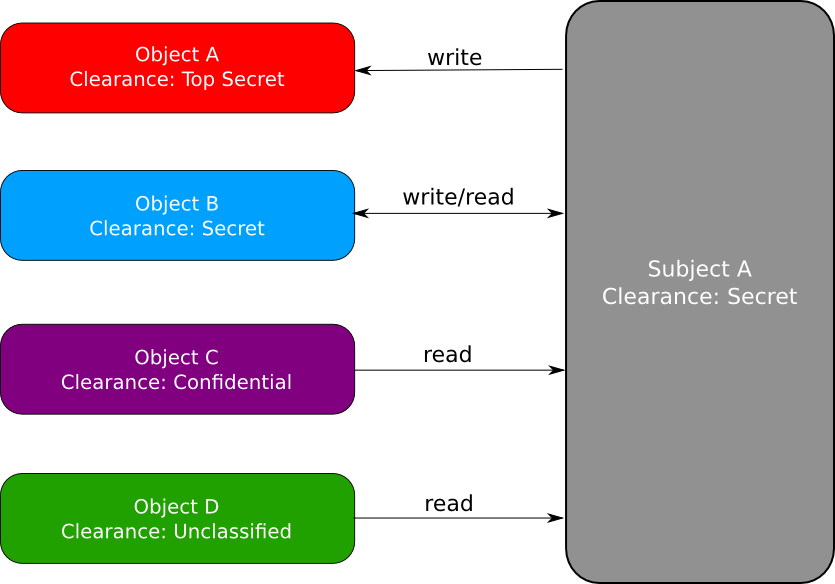
\includegraphics[width=1.0\linewidth]{gfx/chapter_2/blp_security_level_rules}
%\caption[BLP: Security Level rules]{BLP: Security Level read/write  %rules}\label{fig:blp_security_level_rules}
%\end{figure}

In addition to security level labels, as mentioned above, BLP can also be designed in combination with \emph{classification} labels to create a stronger restriction to object accesses.
Under the circumstances, the subject's classification labels should be a subset of the object's to be able gain the access permission.
If we call the subject's roles a set $R1$ and the object's $R2$, where

$$R1, R2 \in \{project manager, programmer, designer\}$$ 

The subject can gain access permission to R2 only if $R1 \subseteq R2$.
\autoref{fig:blp_security_level_roles_rules} shows the principles of handling request from a subject to the other objects regarding only to their security levels.

%\begin{figure}[bth]                                                                                                                                                  
%\myfloatalign
%\includegraphics[width=1.0\linewidth]{gfx/chapter_2/blp_security_level_roles_rules}
%\caption[BLP: A set of Security Level and Roles rules]{BLP: A set of Security %Level and Roles rules}\label{fig:blp_security_level_roles_rules}
%\end{figure}

Finally, a user can use \emph{Discretionary Access Control} (DAC) set the permission to an object.
\cite{centos:2008} cited that MLS access rules are always combined with \emph{conventional access permissions} (or file permission).
It means that if a user with security label \emph{Secret} uses DAC to block access to an object by the other uses, this also block access by by users with security level of \emph{Top Secret}.
Additionally, \cite{bancinco:2015} presented that
\begin{quote}
SELinux MLS policy rules are checked after DAC rules. A higher security clearance does not automatically give permission to arbitrarily browse a file system.
\end{quote}
Hence, \autoref{fig:blp_security_level_roles_rules} will be a mostly complete picture describing about BLP model after we put every components together.

In conclusion, MLS and BLP model, in specification, are suitable for many of real world organization models. It can isolate objects by labeling and protect them in multi-level environment.

\begin{figure}[bth]
\myfloatalign
\subfloat[BLP: Security Level rules]
{\label{fig:blp_security_level_rules}
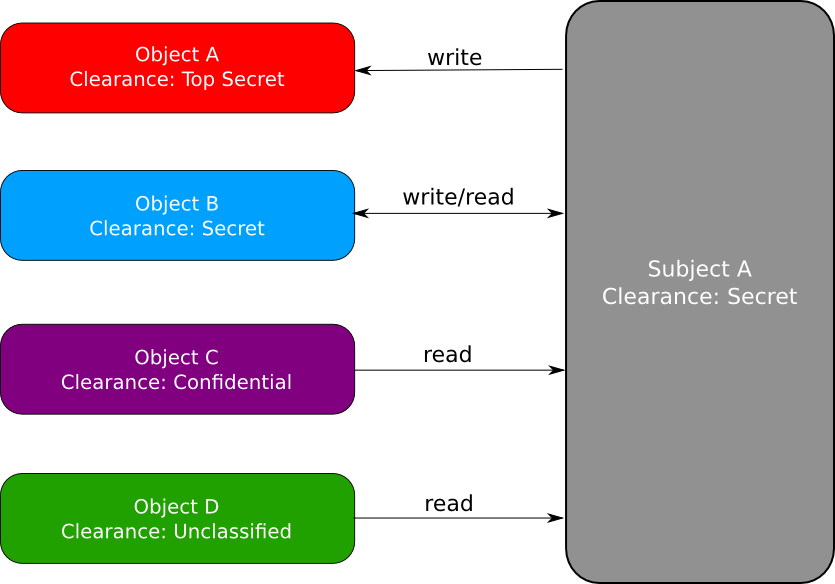
\includegraphics[width=.9\linewidth]{gfx/chapter_2/blp_security_level_rules}} \quad

\subfloat[BLP: A set of Security Level and Roles rules]
{\label{fig:blp_security_level_roles_rules}
\includegraphics[width=.9\linewidth]{gfx/chapter_2/blp_security_level_roles_rules}} \\

\subfloat[BLP: all components illustration]
{\label{fig:blp_example}
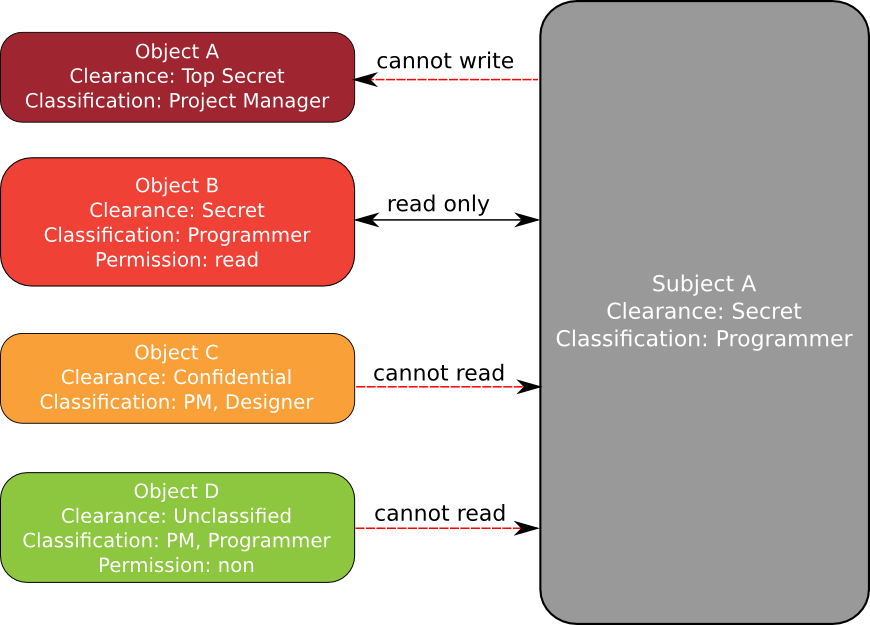
\includegraphics[width=.9\linewidth]{gfx/chapter_2/blp_example}} \\

\caption[BLP illustration]{Illustrate how BLP components form access control}\label{fig:blp_illustration}
\end{figure} 
